\documentclass[11pt]{article}

\usepackage{graphicx}

\title{Locating a Target in Three Dimensions}
\author{Adam Yedidia}

\begin{document}

\maketitle
    
\section{Introduction}

\begin{figure}
\begin{center}
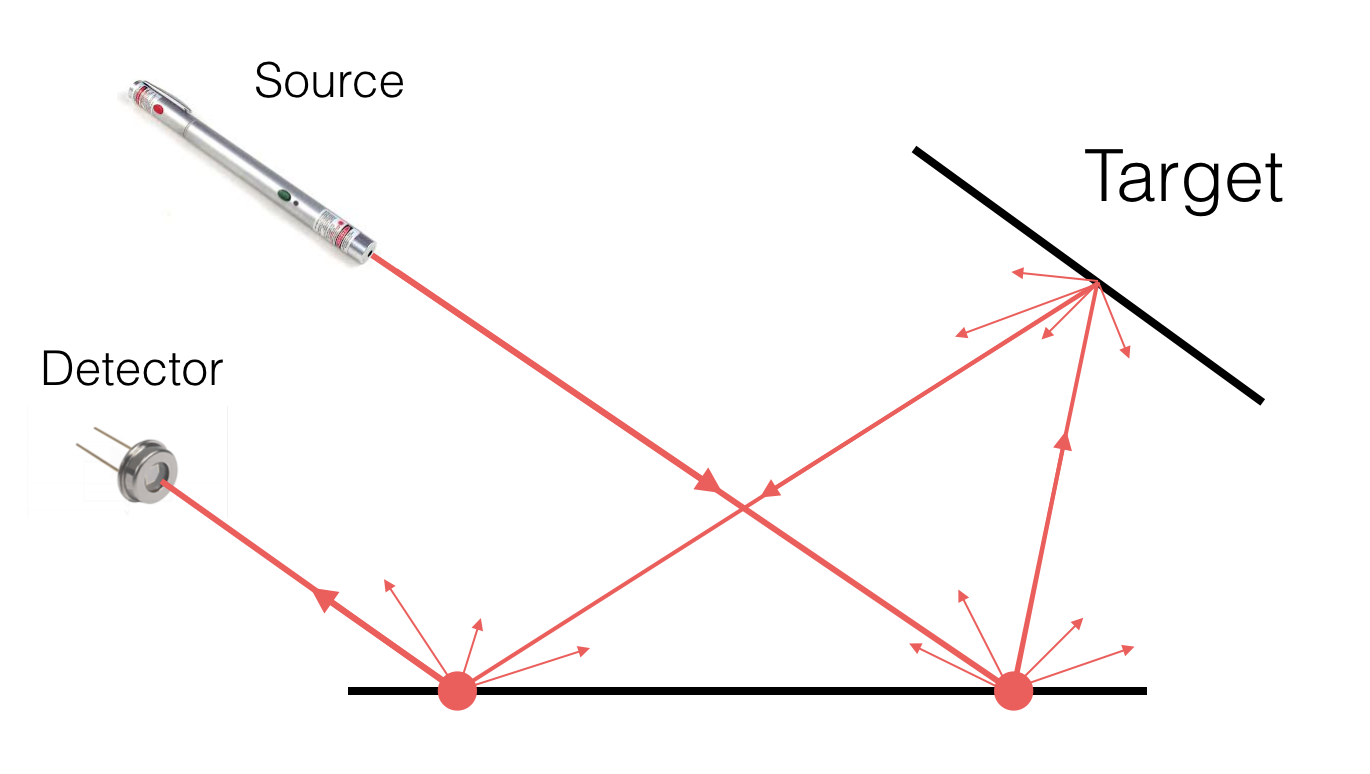
\includegraphics[scale=0.6]{figs/laser.png}
\caption{A view of the problem. Note that while this image is two-dimensional, the real problem I am concerned with is in three dimensions. \label{fig:laser}}
\end{center}
\end{figure}

This is an essay about using the light returns from a directional source and a directional detector\footnotemark~to locate a target in the three-bounce problem. For background on the three-bounce problem, see \emph{On the Localization of Objects Through the Emission and Detection of Light}.
\footnotetext{By a ``directional detector'' I mean a detector that only counts photons that are returning from a specific direction. I will use the term ``point detector'' to describe a detector that counts photons returning from \emph{any} direction (but that does not know the direction from which each photon came). It should be noted that a directional source directed at some point $p$ on a wall is equivalent to a point source of equal intensity directed at that same point $p$, up to glance factors; similarly, a directional detector directed at a point $q$ on a wall is equivalent to a point detector located at that same point $q$, up to glance factors. Therefore, for the sake of convenience in many future figures including Fig.~\ref{fig:twodthreed}, I represent the source and detector as simple point detectors at their locations on the wall; this is, of course, a simplification.}

This writeup is purely concerned with locating a flat surface-shaped target in three dimensions. Two-dimensional models are less interesting because they are qualitatively different: whereas the light bouncing off a three-dimensional target hits many points at once in such a way that all of them reach the detector at the same time, the light bouncing off a two-dimensional target hits only two points at the same time, which completely changes the form of the problem. See Fig.~\ref{fig:twodthreed} for a side-by-side comparison of the two-dimensional and three-dimensional versions of this problem.

\begin{figure}
\begin{center}
\centering
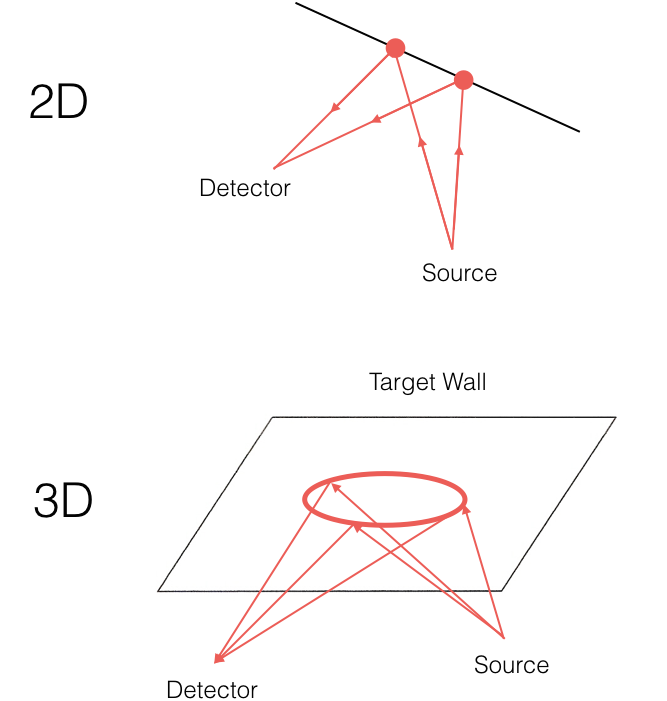
\includegraphics[scale=0.6]{figs/twodthreed.png}
\caption{A side-by-side comparison of a snapshot of the problem in two and in three dimensions. In both versions of the problem, the target is a surface, and the figures show the path taken by the light being received a short time after first light. In the two-dimensional case, the wall is a line, there are two points $p$ on the wall for which the total distance from the source to $p$ to the detector is equal to a given value. In the three-dimensional case, the wall is a plane, and there are infinitely many points $q$ on the wall for which the total distance from the source to $q$ to the detector is equal to a given value. For any given value, these points form an ellipse on the wall, as shown in the diagram. \label{fig:twodthreed}}
\end{center}
\end{figure}

As can be seen in Fig.~\ref{fig:twodthreed}, the points on the wall that mark the paths taken by the light from source to wall to detector form an ellipse. This is because they correspond to the points in three-dimensional space which both are equidistant to the source and the detector, and happen to lie on the plane of the wall. The points in three-dimensional space which are equidistant to two given points $p$ and $q$ form a prolate spheroid\footnotemark, with $p$ and $q$ as its foci; additionally, any cross-section of a prolate spheroid forms an ellipse.

\footnotetext{A \emph{prolate spheroid} is one way of extending the concept of the ellipse into three dimensions. Just as an ellipse can be defined by the lengths of its major and minor axes, so can an ellipsoid be defined by the lengths of its three axes, $a$, $b$, and $c$, with the equation $(\frac{x}{a})^2 + (frac{y}{b})^2 + (frac{z}{c})^2 = r^2$. % TODO make sure that's actually true
If $a$, $b$, and $c$ are all different, that ellipsoid is known as a \emph{triaxial ellipsoid}. If $a = b$ and $c < a$ and $b$, that ellipsoid is called an \emph{oblate spheroid}, and has a shape like that of a Chinese bean pastry. If $a = b$ and $c > a$ and $b$, that ellipsoid is called a \emph{prolate spheroid}, and has a shape more like that of a baguette. Finally, of course, if $a = b = c$, the ellipsoid is a sphere. Although every circle has one focus, and every non-circular ellipse has two foci, not every non-spherical ellipsoid has two foci; indeed, only prolate spheroids have two foci, and only they can be described as the set of points in three dimensions equidistant from their two foci. Therefore, it is prolate spheroids that interest us in this problem, to the exclusion of other ellipsoids, because our interest is derived from the fact that we are interested in the set of points equidistant from the source and the detector.}

\section{A Forward Model}

First, we will direct our interest towards the problem of efficiently computing the pattern of the light returns, as a function of the location of the target. As it turns out, computing the light returns from the target's location is a problem that can be solved in closed form.

Recall that the target is a plane. We therefore need three degrees of freedom to fully specify the plane's location and orientation. We can see this from the fact that the equation for a plane (using Cartesian coordinates) is $ax + by + cz = d$, with four degrees of freedom $a, b, c,$ and $d$, but with one redundant degree of freedom arising from the fact that the equation for the plane can be scaled without changing the plane's form. 

An alternate way of deriving the form of a plane from three specified values, which will turn out to be very convenient for this problem, is to specify the location of a single point, which is presumed to be the point of contact with the wall through which first light reaches the detector from the source. Because it's the point of \emph{first} contact, it is necessarily tangent to the prolate spheroid defined with the detector and source locations as its foci (that prolate spheroid describes the set of points that have the smallest total distance from the detector and source, that could still possibly intersect the target's plane). In this way, any plane can be described, with the exception of planes intersecting the line segment linking source and detector. These planes are of no interest to us in any case, because there would be no way to shoot a beam of light from the source to them to the detector without going \emph{through} the plane. (We presume the target plane is opaque.)

Let's try converting from one of these schemes for describing planes to the other, for the sake of illustration. Imagine our source point (the point at which the directional source hits the reflecting wall) is at $(-l,0,0)$, and our detector point (the point at which the directional detector watches the reflecting wall) is at $(l,0,0)$. Therefore, we're likely to find it particularly useful to describe this plane in terms of what point on it is tangent to a prolate spheroid with foci $(-l,0,0)$ and $(l,0,0)$. 

Let's suppose that that the plane is tangent to a prolate spheroid with those foci at the point $(x_p,y_p,z_p)$. We know that at that point, the partial derivatives of the equation for the spheroid and that for the plane should be equal. Call the major and minor axes of the prolate spheroid $A$ and $B$ respectively. If we'd like to describe this plane with a traditional Cartesian equation, $ax + by + cz = d$, then we know that the equation for the spheroid, $\frac{x^2}{A^2} + \frac{y^2}{B^2} + \frac{z^2}{B^2} = $



\end{document}